\documentclass{book}

\usepackage{listings}
\usepackage{theorem}
\usepackage{graphicx}
\usepackage{hyperref}
\usepackage{amsfonts}
\usepackage{amsmath}
\usepackage[table]{xcolor}
\usepackage{array,calc}
\usepackage{amsmath}

\newtheorem{exercise}{Exercise}


\lstset{
  language=Java,
  basicstyle=\ttfamily\footnotesize,
  numbers = left
}

\newcommand{\co}[1]{\lstinline[language=Java, basicstyle=\ttfamily]{#1}}

\begin{document}

\chapter{ImageJ}
ImageJ is a Java library for digital image analysis and processing. The library contains interfaces and classes for creating, modifying and displaying images. In this chapter, we explain how to perform basic image operations using this library.

\section{Setting up ImageJ}
ImageJ is a library for \emph{Java}. In the remainder of this section, we assume that a Java Development Kit (version 6 or higher) and the Eclipse integrated development environment are installed on your machine. If Java is not installed on your machine, download and install a Java Development Kit from \href{http://www.oracle.com/technetwork/java/javase/downloads/index.html}{http://www.oracle.com/technetwork/java/javase/downloads/index.html}. Similarly, if the Eclipse IDE is not installed on your machine, download and install it from \href{http://www.eclipse.org/}{http://www.eclipse.org/}.

The ImageJ implementation, tutorials and additional documentation are available online at \href{http://rsbweb.nih.gov/ij}{http://rsbweb.nih.gov/ij}. To install ImageJ, download the platform independent release from \href{http://rsbweb.nih.gov/ij/download.html}{http://rsbweb.nih.gov/ij/download.html}. Extract the zip file to a location of your choice.

ImageJ can be used both as a standalone application and as a library. To run the application,  execute ImageJ.exe (on Windows) or ImageJ.app (on Mac). After starting the application, the following graphical user interface should be displayed on your screen:

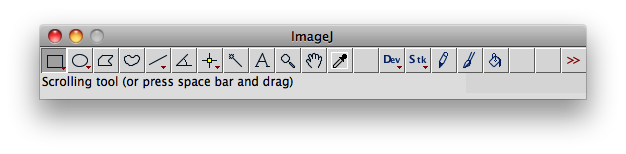
\includegraphics[scale=0.5]{ImageJ-screenshot.png}

\begin{exercise}
Experiment with the ImageJ graphical user interface:
\begin{itemize}
  \item Open \texttt{lena.png} via \texttt{File>Open...}.
  \item \texttt{lena.png} is an rgb color image. However, we will first explain most image processing techniques using gray scale images. Convert the image to 8 bit gray scale via \texttt{Image>Type>8-bit}.
  \item A gray scale image is a function from coordinates to colors in the range 0 to 255. Visualise this function via  \texttt{Plugins>3D>Interactive 3D Surface Plot}. 
  \item Detect edges in the image via \texttt{Process>Find Edges}. Later in this course, we will explain how edge detection works and how it can be used to sharpen images and to perform seam carving.
\end{itemize} 
\end{exercise}

The ImageJ library is packaged as a jar file called \texttt{ij.jar}. This jar file is located in the ImageJ directory. To use the interfaces and classes provided by ImageJ, \texttt{ij.jar} must be included in the classpath when compiling and running any program that uses the library. 

\begin{exercise}
Set up Eclipse as follows:
\begin{itemize}
  \item Start Eclipse and create a new Java project called \texttt{digitalimageprocessing}.
  \item Add \texttt{ij.jar} to the classpath by right-clicking the project and selecting \texttt{Build Path>Add External Archives ...} as shown below.
  \begin{center}
  \includegraphics[scale=0.25]{eclipse-classpath.png}
  \end{center}
  After adding \texttt{ij.jar} to the classpath, the project should contain a new item called \texttt{Referenced Libraries}. This item contains \texttt{ij.jar} as a subitem. 
  \item To access the ImageJ API documentation directly in Eclipse, right-click \texttt{ij.jar} in Eclipse and select \texttt{Properties} and click \texttt{Javadoc Location}. Enter \href{http://rsbweb.nih.gov/ij/developer/api/}{http://rsbweb.nih.gov/ij/developer/api/} as the \texttt{Javadoc location path} and click \texttt{OK}.  
\end{itemize}
\end{exercise}

\section{Images}
An image is a rectangular, two-dimensional grid of pixels, where each pixel represents the color at that location. In ImageJ, images are represented as objects of the class \texttt{ImagePlus}. This class provides methods for querying the image's width, height, pixel values, etc. 

\subsection{Opening images}
The easiest way to open an image is to call the constructor of ImagePlus as follows:
\begin{lstlisting}
ImagePlus image = new ImagePlus("lena.png");
\end{lstlisting}
The argument of this constructor is the url of the image file. This url can refer to a file on disk or to a network location. If the file cannot be accessed or is not a valid image, the constructor prints an error message on standard out.

\begin{exercise}
Open an image and display its size. To do so, create a new class named \texttt{MyFirstImageProcessor} in the default package. Add a \texttt{main} method to this class that first opens the image located at  [TODO] and then prints the image's width and height using respectively the methods \co{getWidth} and \co{getHeight}.
\end{exercise}

\subsection{Displaying images}
Images can be displayed via an \texttt{ImageWindow} as follows:
\begin{lstlisting}
ImagePlus image = new ImagePlus("lena.png");
ImageWindow window = new ImageWindow(image);
window.setVisible(true);
\end{lstlisting}
\begin{exercise}
Make the \texttt{main} method of the class \texttt{MyFirstImageProcessor} display the image in a window.
\end{exercise}

\subsection{Modifying images}
Images can be modified via an \texttt{ImageProcessor}. The key methods of this class are \texttt{getPixel} and \texttt{putPixel}. These methods respectively return and modify the pixel value (as an integer) at a given location. For gray scale images, the pixel value is an integer in the range 0 (representing black) to 255 (representing white). For RGB color images, the pixel value is the integer encoding of the separate color components.  For example, the code snippet shown below inverts a gray scale image. That is, white pixels become black and vice versa, black pixels become white.

\begin{lstlisting}
ImagePlus image = new ImagePlus("lena-gray.png");
ImageProcessor ip = image.getProcessor();
for(int x = 0; x < ip.getWidth(); x++) {
  for(int y = 0; y < ip.getHeight(); y++) {
    int grayColor = ip.getPixel(x, y);
    ip.putPixel(x, y, 255 - grayColor);
  }  
}
\end{lstlisting}

\begin{exercise}\label{ex:invert}
Write a class \texttt{ImageInvertor} that inverts gray scale images based on the code snippet shown on above. The output for \texttt{lena-gray.png} should look as follows:
\begin{center}
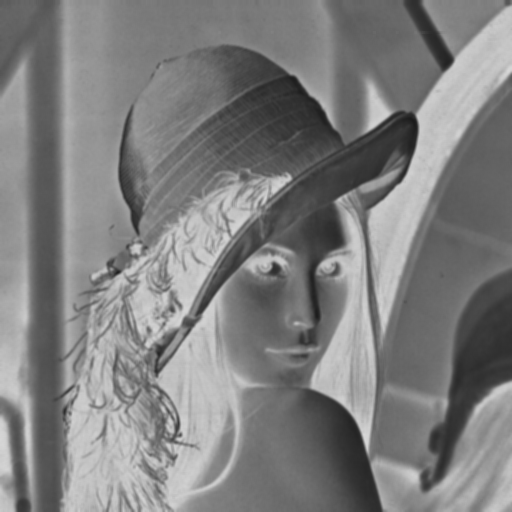
\includegraphics[scale=0.2]{lena-gray-inverted.png}
\end{center}
\end{exercise}

\begin{exercise}\label{ex:flipper}
Write a class  \texttt{ImageFlipper} that flips an image vertically (i.e. puts the image upside down). For example, the output for \texttt{lena.png} should look as follows:
\begin{center}
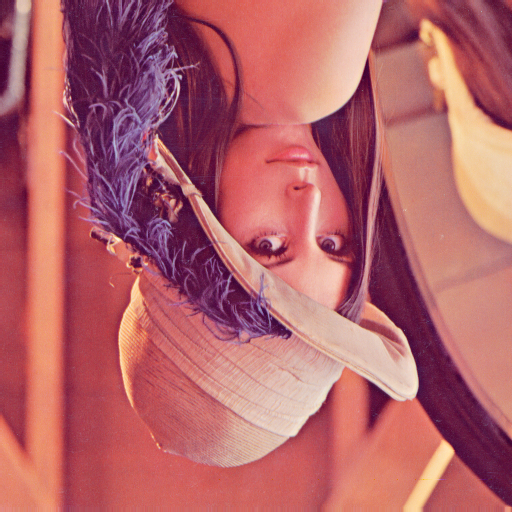
\includegraphics[scale=0.2]{lena-flipped-hor.png}
\end{center}
\end{exercise}

\begin{exercise}
Modify the class \texttt{ImageInvertor} from Exercise~\ref{ex:invert} such that it can handle RGB color images.
\begin{itemize}
  \item Implement a method \co{getRGBComponentsFromInt} that converts an integer into an array containing the RGB components.
  \item Implement a method \co{getIntFromRGBComponents} that converts an array of RGB components into an integer.
  \item Modify the \texttt{main} method of \texttt{ImageInvertor}  such that it checks whether the image is gray scale or RGB color. You can use the method [todo]\texttt{} to do so. If the image is gray scale, the existing code should be used for inverting the image. If the image is RGB color, then for each pixel each  color components should be inverted separately. Use the methods \co{getRGBComponentsFromInt} and \co{getIntFromRGBComponents} to help you out.
\end{itemize}
The output of \texttt{ImageInvertor} for \texttt{lena.png} should look as follows:
\begin{center}
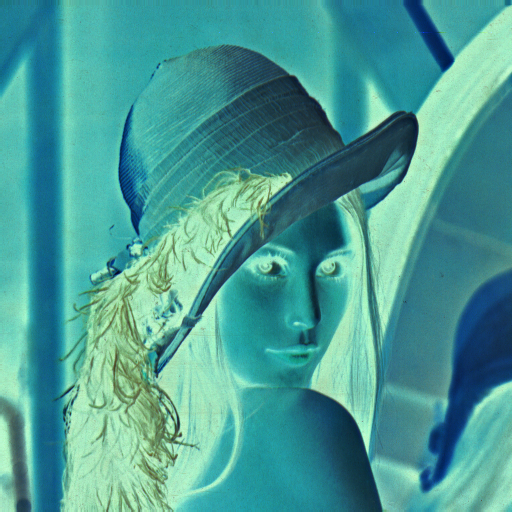
\includegraphics[scale=0.2]{lena-inverted.png}
\end{center}
\end{exercise}

\subsection{Saving images}
In addition to displaying images on screen, we often want to save them to disk. The code shown below makes use of the static method \co{ImageIO.write} to save \co{img} to \co{output.png} in the png file format.
\begin{lstlisting}
ImagePlus img = ...;
ImageIO.write(img.getBufferedImage(), "png", 
  new File("output.png"));
\end{lstlisting}
Note that \texttt{ImageIO.write} throws \texttt{IOException} when writing the image fails. For example, writing can fail because the current user does not have write permission or because the file is in use by another application.

\begin{exercise}
Modify the class \texttt{ImageFlipper} from Exercise~\ref{ex:flipper} such that it saves the flipped image to disk to \texttt{out.png}. The application should not crash when \co{ImageIO.write} fails, but instead write an error message to standard output (i.e.  \texttt{System.out}).
\end{exercise}

\section{Getting user input}
In all but the simplest applications, user input is required. For example, 

\subsection{Command line arguments}

\subsection{Standard input}

\subsection{GenericDialog}

\subsection{Swing}


%What happens if you set the color to -1 for a grayscale image?
%What happens if you get or put a pixel outside of the image?

\section{ImageJ Plugins}


\begin{exercise}
  item
\end{exercise}
% access exif info in IJ?
\end{document}